\documentclass{standalone}
\usepackage[utf8]{inputenc}
\usepackage{tikz}

\begin{document}

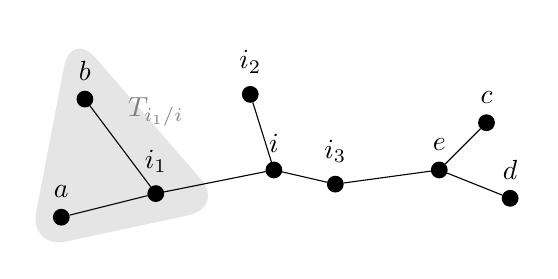
\begin{tikzpicture}[scale=.6]
 \draw[rounded corners=5mm, fill=gray!20, draw=white] (-.7,-.2) -- (3.5,0.7) -- (0.2,4.5) -- cycle;
  \node[label={[gray]$T_{i_1/i}$}] (Ti1i) at (2,2) {}; 
  \begin{scope}[every node/.style={circle,draw=black,fill= black,minimum size=3.5pt, inner sep=2}];
  \node[label=$a$] (a) at (0,0.5) {};
  \node[label=$b$] (b) at (0.5,3) {};
  \node[label=$c$] (c) at (9,2.5) {};
  \node[label=$d$] (d) at (9.5,0.9) {};
  \node[label=$i_1$] (i1) at (2,1) {};
  \node[label=$i_2$] (i2) at (4,3.1) {};
  \node[label=$i_3$] (i3) at (5.8,1.2) {};
  \node[label=$i$] (i) at (4.5,1.5) {};
  \node[label=$e$] (e) at (8,1.5) {};
  \end{scope}
  \draw (a) -- (i1) -- (b);
  \draw (i1) -- (i) -- (i3) -- (e) -- (c);
  \draw (e) -- (d); 
  \draw (i) -- (i2);
   \end{tikzpicture}
  \end{document}
